% Created by tikzDevice version 0.10.1 on 2018-01-23 02:21:41
% !TEX encoding = UTF-8 Unicode
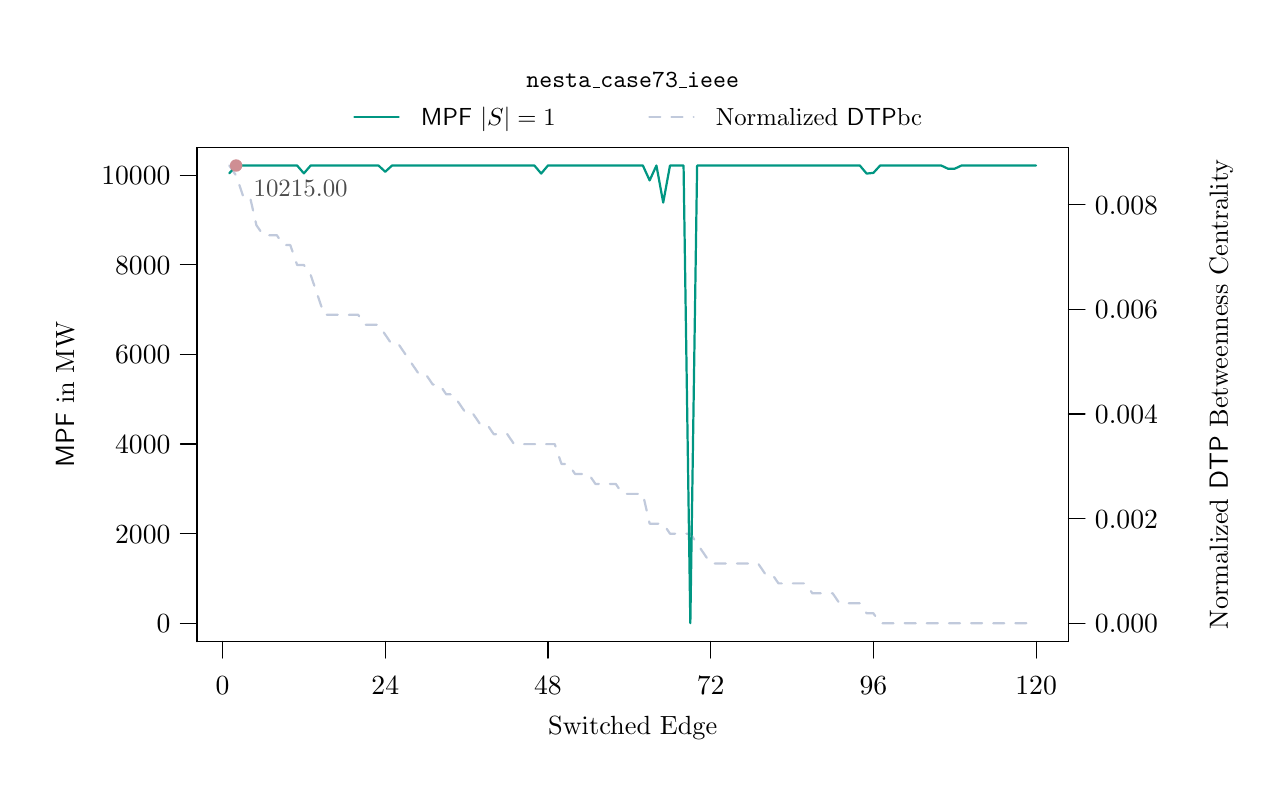
\begin{tikzpicture}[x=1pt,y=1pt]
\definecolor{fillColor}{RGB}{255,255,255}
\path[use as bounding box,fill=fillColor,fill opacity=0.00] (0,0) rectangle (440.85,271.01);
\begin{scope}
\path[clip] (  0.00,  0.00) rectangle (440.85,271.01);
\definecolor{drawColor}{RGB}{193,202,220}

\path[draw=drawColor,line width= 0.8pt,dash pattern=on 4pt off 4pt ,line join=round,line cap=round] ( 72.86,221.20) --
	( 75.31,217.60) --
	( 77.76,210.41) --
	( 80.21,210.41) --
	( 82.66,199.63) --
	( 85.11,196.03) --
	( 87.56,196.03) --
	( 90.01,196.03) --
	( 92.46,192.44) --
	( 94.91,192.44) --
	( 97.36,185.24) --
	( 99.81,185.24) --
	(102.26,181.65) --
	(104.71,174.46) --
	(107.16,167.27) --
	(109.61,167.27) --
	(112.06,167.27) --
	(114.51,167.27) --
	(116.96,167.27) --
	(119.41,167.27) --
	(121.86,163.67) --
	(124.31,163.67) --
	(126.76,163.67) --
	(129.21,160.08) --
	(131.66,156.48) --
	(134.11,156.48) --
	(136.56,152.89) --
	(139.01,149.29) --
	(141.46,145.70) --
	(143.90,145.70) --
	(146.35,142.10) --
	(148.80,142.10) --
	(151.25,138.51) --
	(153.70,138.51) --
	(156.15,134.91) --
	(158.60,131.32) --
	(161.05,131.32) --
	(163.50,127.72) --
	(165.95,127.72) --
	(168.40,124.13) --
	(170.85,124.13) --
	(173.30,124.13) --
	(175.75,120.53) --
	(178.20,120.53) --
	(180.65,120.53) --
	(183.10,120.53) --
	(185.55,120.53) --
	(188.00,120.53) --
	(190.45,120.53) --
	(192.90,113.34) --
	(195.35,113.34) --
	(197.80,109.74) --
	(200.25,109.74) --
	(202.70,109.74) --
	(205.15,106.15) --
	(207.60,106.15) --
	(210.05,106.15) --
	(212.50,106.15) --
	(214.95,102.55) --
	(217.40,102.55) --
	(219.85,102.55) --
	(222.30,102.55) --
	(224.75, 91.77) --
	(227.20, 91.77) --
	(229.65, 91.77) --
	(232.10, 88.17) --
	(234.55, 88.17) --
	(237.00, 88.17) --
	(239.45, 88.17) --
	(241.90, 84.58) --
	(244.35, 80.98) --
	(246.80, 77.39) --
	(249.25, 77.39) --
	(251.70, 77.39) --
	(254.15, 77.39) --
	(256.60, 77.39) --
	(259.05, 77.39) --
	(261.49, 77.39) --
	(263.94, 77.39) --
	(266.39, 73.79) --
	(268.84, 73.79) --
	(271.29, 70.20) --
	(273.74, 70.20) --
	(276.19, 70.20) --
	(278.64, 70.20) --
	(281.09, 70.20) --
	(283.54, 66.60) --
	(285.99, 66.60) --
	(288.44, 66.60) --
	(290.89, 66.60) --
	(293.34, 63.01) --
	(295.79, 63.01) --
	(298.24, 63.01) --
	(300.69, 63.01) --
	(303.14, 59.41) --
	(305.59, 59.41) --
	(308.04, 55.82) --
	(310.49, 55.82) --
	(312.94, 55.82) --
	(315.39, 55.82) --
	(317.84, 55.82) --
	(320.29, 55.82) --
	(322.74, 55.82) --
	(325.19, 55.82) --
	(327.64, 55.82) --
	(330.09, 55.82) --
	(332.54, 55.82) --
	(334.99, 55.82) --
	(337.44, 55.82) --
	(339.89, 55.82) --
	(342.34, 55.82) --
	(344.79, 55.82) --
	(347.24, 55.82) --
	(349.69, 55.82) --
	(352.14, 55.82) --
	(354.59, 55.82) --
	(357.04, 55.82) --
	(359.49, 55.82) --
	(361.94, 55.82) --
	(364.39, 55.82);
\end{scope}
\begin{scope}
\path[clip] (  0.00,  0.00) rectangle (440.85,271.01);
\definecolor{drawColor}{RGB}{0,0,0}

\path[draw=drawColor,line width= 0.4pt,line join=round,line cap=round] ( 61.20, 49.20) --
	(376.05, 49.20) --
	(376.05,227.81) --
	( 61.20,227.81) --
	( 61.20, 49.20);
\end{scope}
\begin{scope}
\path[clip] (  0.00,  0.00) rectangle (440.85,271.01);
\definecolor{drawColor}{RGB}{0,0,0}

\path[draw=drawColor,line width= 0.4pt,line join=round,line cap=round] (376.05, 55.82) -- (376.05,206.99);

\path[draw=drawColor,line width= 0.4pt,line join=round,line cap=round] (376.05, 55.82) -- (382.05, 55.82);

\path[draw=drawColor,line width= 0.4pt,line join=round,line cap=round] (376.05, 93.61) -- (382.05, 93.61);

\path[draw=drawColor,line width= 0.4pt,line join=round,line cap=round] (376.05,131.40) -- (382.05,131.40);

\path[draw=drawColor,line width= 0.4pt,line join=round,line cap=round] (376.05,169.20) -- (382.05,169.20);

\path[draw=drawColor,line width= 0.4pt,line join=round,line cap=round] (376.05,206.99) -- (382.05,206.99);

\node[text=drawColor,anchor=base west,inner sep=0pt, outer sep=0pt, scale=  1.00] at (385.65, 52.37) {0.000};

\node[text=drawColor,anchor=base west,inner sep=0pt, outer sep=0pt, scale=  1.00] at (385.65, 90.17) {0.002};

\node[text=drawColor,anchor=base west,inner sep=0pt, outer sep=0pt, scale=  1.00] at (385.65,127.96) {0.004};

\node[text=drawColor,anchor=base west,inner sep=0pt, outer sep=0pt, scale=  1.00] at (385.65,165.75) {0.006};

\node[text=drawColor,anchor=base west,inner sep=0pt, outer sep=0pt, scale=  1.00] at (385.65,203.55) {0.008};
\end{scope}
\begin{scope}
\path[clip] (  0.00,  0.00) rectangle (440.85,271.01);
\definecolor{drawColor}{RGB}{0,150,130}

\path[draw=drawColor,line width= 0.8pt,line join=round,line cap=round] ( 72.86,218.36) --
	( 75.31,221.20) --
	( 77.76,221.20) --
	( 80.21,221.20) --
	( 82.66,221.20) --
	( 85.11,221.20) --
	( 87.56,221.20) --
	( 90.01,221.20) --
	( 92.46,221.20) --
	( 94.91,221.20) --
	( 97.36,221.20) --
	( 99.81,218.36) --
	(102.26,221.20) --
	(104.71,221.20) --
	(107.16,221.20) --
	(109.61,221.20) --
	(112.06,221.20) --
	(114.51,221.20) --
	(116.96,221.20) --
	(119.41,221.20) --
	(121.86,221.20) --
	(124.31,221.20) --
	(126.76,221.20) --
	(129.21,218.95) --
	(131.66,221.20) --
	(134.11,221.20) --
	(136.56,221.20) --
	(139.01,221.20) --
	(141.46,221.20) --
	(143.90,221.20) --
	(146.35,221.20) --
	(148.80,221.20) --
	(151.25,221.20) --
	(153.70,221.20) --
	(156.15,221.20) --
	(158.60,221.20) --
	(161.05,221.20) --
	(163.50,221.20) --
	(165.95,221.20) --
	(168.40,221.20) --
	(170.85,221.20) --
	(173.30,221.20) --
	(175.75,221.20) --
	(178.20,221.20) --
	(180.65,221.20) --
	(183.10,221.20) --
	(185.55,218.29) --
	(188.00,221.20) --
	(190.45,221.20) --
	(192.90,221.20) --
	(195.35,221.20) --
	(197.80,221.20) --
	(200.25,221.20) --
	(202.70,221.20) --
	(205.15,221.20) --
	(207.60,221.20) --
	(210.05,221.20) --
	(212.50,221.20) --
	(214.95,221.20) --
	(217.40,221.20) --
	(219.85,221.20) --
	(222.30,221.20) --
	(224.75,215.81) --
	(227.20,221.20) --
	(229.65,207.80) --
	(232.10,221.20) --
	(234.55,221.20) --
	(237.00,221.20) --
	(239.45, 55.82) --
	(241.90,221.20) --
	(244.35,221.20) --
	(246.80,221.20) --
	(249.25,221.20) --
	(251.70,221.20) --
	(254.15,221.20) --
	(256.60,221.20) --
	(259.05,221.20) --
	(261.49,221.20) --
	(263.94,221.20) --
	(266.39,221.20) --
	(268.84,221.20) --
	(271.29,221.20) --
	(273.74,221.20) --
	(276.19,221.20) --
	(278.64,221.20) --
	(281.09,221.20) --
	(283.54,221.20) --
	(285.99,221.20) --
	(288.44,221.20) --
	(290.89,221.20) --
	(293.34,221.20) --
	(295.79,221.20) --
	(298.24,221.20) --
	(300.69,221.20) --
	(303.14,218.29) --
	(305.59,218.53) --
	(308.04,221.20) --
	(310.49,221.20) --
	(312.94,221.20) --
	(315.39,221.20) --
	(317.84,221.20) --
	(320.29,221.20) --
	(322.74,221.20) --
	(325.19,221.20) --
	(327.64,221.20) --
	(330.09,221.20) --
	(332.54,220.05) --
	(334.99,220.05) --
	(337.44,221.20) --
	(339.89,221.20) --
	(342.34,221.20) --
	(344.79,221.20) --
	(347.24,221.20) --
	(349.69,221.20) --
	(352.14,221.20) --
	(354.59,221.20) --
	(357.04,221.20) --
	(359.49,221.20) --
	(361.94,221.20) --
	(364.39,221.20);
\end{scope}
\begin{scope}
\path[clip] (  0.00,  0.00) rectangle (440.85,271.01);
\definecolor{drawColor}{RGB}{0,0,0}

\path[draw=drawColor,line width= 0.4pt,line join=round,line cap=round] ( 61.20, 49.20) --
	(376.05, 49.20) --
	(376.05,227.81) --
	( 61.20,227.81) --
	( 61.20, 49.20);
\end{scope}
\begin{scope}
\path[clip] (  0.00,  0.00) rectangle (440.85,271.01);
\definecolor{drawColor}{RGB}{0,0,0}

\path[draw=drawColor,line width= 0.4pt,line join=round,line cap=round] ( 61.20, 55.82) -- ( 61.20,217.72);

\path[draw=drawColor,line width= 0.4pt,line join=round,line cap=round] ( 61.20, 55.82) -- ( 55.20, 55.82);

\path[draw=drawColor,line width= 0.4pt,line join=round,line cap=round] ( 61.20, 88.20) -- ( 55.20, 88.20);

\path[draw=drawColor,line width= 0.4pt,line join=round,line cap=round] ( 61.20,120.58) -- ( 55.20,120.58);

\path[draw=drawColor,line width= 0.4pt,line join=round,line cap=round] ( 61.20,152.96) -- ( 55.20,152.96);

\path[draw=drawColor,line width= 0.4pt,line join=round,line cap=round] ( 61.20,185.34) -- ( 55.20,185.34);

\path[draw=drawColor,line width= 0.4pt,line join=round,line cap=round] ( 61.20,217.72) -- ( 55.20,217.72);

\node[text=drawColor,anchor=base east,inner sep=0pt, outer sep=0pt, scale=  1.00] at ( 51.60, 52.37) {0};

\node[text=drawColor,anchor=base east,inner sep=0pt, outer sep=0pt, scale=  1.00] at ( 51.60, 84.75) {2000};

\node[text=drawColor,anchor=base east,inner sep=0pt, outer sep=0pt, scale=  1.00] at ( 51.60,117.13) {4000};

\node[text=drawColor,anchor=base east,inner sep=0pt, outer sep=0pt, scale=  1.00] at ( 51.60,149.51) {6000};

\node[text=drawColor,anchor=base east,inner sep=0pt, outer sep=0pt, scale=  1.00] at ( 51.60,181.89) {8000};

\node[text=drawColor,anchor=base east,inner sep=0pt, outer sep=0pt, scale=  1.00] at ( 51.60,214.27) {10000};
\end{scope}
\begin{scope}
\path[clip] (  0.00,  0.00) rectangle (440.85,271.01);
\definecolor{fillColor}{RGB}{207,142,147}

\path[fill=fillColor] ( 75.31,221.20) circle (  2.25);
\end{scope}
\begin{scope}
\path[clip] (  0.00,  0.00) rectangle (440.85,271.01);
\definecolor{drawColor}{RGB}{0,0,0}

\path[draw=drawColor,line width= 0.4pt,line join=round,line cap=round] ( 61.20, 49.20) --
	(376.05, 49.20) --
	(376.05,227.81) --
	( 61.20,227.81) --
	( 61.20, 49.20);
\end{scope}
\begin{scope}
\path[clip] (  0.00,  0.00) rectangle (440.85,271.01);
\definecolor{drawColor}{gray}{0.30}

\node[text=drawColor,anchor=base,inner sep=0pt, outer sep=0pt, scale=  0.90] at ( 98.63,210.04) {10215.00};
\end{scope}
\begin{scope}
\path[clip] (  0.00,  0.00) rectangle (440.85,271.01);
\definecolor{drawColor}{RGB}{0,0,0}

\path[draw=drawColor,line width= 0.4pt,line join=round,line cap=round] ( 70.41, 49.20) -- (364.39, 49.20);

\path[draw=drawColor,line width= 0.4pt,line join=round,line cap=round] ( 70.41, 49.20) -- ( 70.41, 43.20);

\path[draw=drawColor,line width= 0.4pt,line join=round,line cap=round] (129.21, 49.20) -- (129.21, 43.20);

\path[draw=drawColor,line width= 0.4pt,line join=round,line cap=round] (188.00, 49.20) -- (188.00, 43.20);

\path[draw=drawColor,line width= 0.4pt,line join=round,line cap=round] (246.80, 49.20) -- (246.80, 43.20);

\path[draw=drawColor,line width= 0.4pt,line join=round,line cap=round] (305.59, 49.20) -- (305.59, 43.20);

\path[draw=drawColor,line width= 0.4pt,line join=round,line cap=round] (364.39, 49.20) -- (364.39, 43.20);

\node[text=drawColor,anchor=base,inner sep=0pt, outer sep=0pt, scale=  1.00] at ( 70.41, 30.00) {0};

\node[text=drawColor,anchor=base,inner sep=0pt, outer sep=0pt, scale=  1.00] at (129.21, 30.00) {24};

\node[text=drawColor,anchor=base,inner sep=0pt, outer sep=0pt, scale=  1.00] at (188.00, 30.00) {48};

\node[text=drawColor,anchor=base,inner sep=0pt, outer sep=0pt, scale=  1.00] at (246.80, 30.00) {72};

\node[text=drawColor,anchor=base,inner sep=0pt, outer sep=0pt, scale=  1.00] at (305.59, 30.00) {96};

\node[text=drawColor,anchor=base,inner sep=0pt, outer sep=0pt, scale=  1.00] at (364.39, 30.00) {120};

\node[text=drawColor,anchor=base,inner sep=0pt, outer sep=0pt, scale=  0.95] at (218.62, 15.60) {Switched Edge};

\node[text=drawColor,rotate= 90.00,anchor=base,inner sep=0pt, outer sep=0pt, scale=  0.95] at ( 16.80,138.51) {$\mathsf{MPF}$ in~$\mathrm{MW}$};

\node[text=drawColor,rotate= 90.00,anchor=base,inner sep=0pt, outer sep=0pt, scale=  0.95] at (433.65,138.51) {Normalized~$\mathsf{DTP}$ Betweenness Centrality};
\end{scope}
\begin{scope}
\path[clip] (  0.00,  0.00) rectangle (440.85,271.01);
\definecolor{drawColor}{RGB}{0,150,130}

\path[draw=drawColor,line width= 0.8pt,line join=round,line cap=round] (118.04,238.60) -- (134.06,238.60);
\definecolor{drawColor}{RGB}{193,202,220}

\path[draw=drawColor,line width= 0.8pt,dash pattern=on 4pt off 4pt ,line join=round,line cap=round] (224.63,238.60) -- (240.65,238.60);
\definecolor{drawColor}{RGB}{0,0,0}

\node[text=drawColor,anchor=base,inner sep=0pt, outer sep=0pt, scale=  0.89] at (218.62,249.28) {\texttt{nesta\_case73\_ieee}};

\node[text=drawColor,anchor=base west,inner sep=0pt, outer sep=0pt, scale=  0.89] at (142.07,235.54) {$\mathsf{MPF}~|S|=1$};

\node[text=drawColor,anchor=base west,inner sep=0pt, outer sep=0pt, scale=  0.89] at (248.66,235.54) {Normalized~$\mathsf{DTP}$bc};
\end{scope}
\end{tikzpicture}
